\documentclass[10pt]{article}
\usepackage[T1]{fontenc}
\usepackage[utf8]{inputenc}
\usepackage[margin=0.7in]{geometry}
\usepackage{graphicx}
\usepackage{booktabs}
\usepackage{amsmath}
\usepackage{amssymb}
\usepackage{array}
\usepackage{caption}
\captionsetup{font=small}
\usepackage[hidelinks]{hyperref}
\usepackage{titlesec}
\titleformat*{\section}{\large\bfseries}
\titleformat*{\subsection}{\normalsize\bfseries}
\setlength{\parskip}{0.15em}
\graphicspath{{./}{figures/}}

\title{\textbf{An Autonomous Medicinal-Chemistry Scientist for Payload-Aware Antibody-Conjugate Linker Design: the Derived Rule Reads the Literature, Designs the Molecule, and Knows When the Field Disagrees}}
\author{Elia Savino$^{1,d}$, Joshua W.\ Sin$^{2,3,d}$, Morgan G.\ L.\ Reigner$^{1,d}$, Miqu\`el \`A.\ P\'erez-Puigdom\`enech$^{2,d}$, Derk H.\ W.\ ten Klooster$^{1,d}$, Claude$^{d}$, J.A.R.V.I.S$^{d}$}
\date{}
\begin{document}
\maketitle
\begin{center}\footnotesize $^{1}$No\"el Research Group, Van 't Hoff Institute for Molecular Sciences, University of Amsterdam. $^{2}$Laboratory of Artificial Chemical Intelligence (LIAC), EPFL. $^{3}$Process Chemistry \& Catalysis, F.\ Hoffmann-La Roche AG, Basel. $^{d}$All authors contributed equally.\end{center}
\begin{abstract}The right antibody-conjugate linker inverts with the payload, and an autonomous agent should not merely \emph{apply} that logic but \emph{derive} it from the literature, let it \emph{drive} molecular design, and report its own confidence---including when the field disagrees. We read 31 primary papers with a retrieval-grounded LLM, emit an auditable reasoning chain (retrieved passages $\rightarrow$ grounded exemplars $\rightarrow$ derived rule $+$ confidence $\rightarrow$ compiled objective), and---closing the central gap of the prior iteration---use that compiled objective to \emph{generate} the linkers with REINVENT4 LinkInvent, so the delivered molecules are produced by the agent's reasoning and carry the class-specific motif (Val-Cit for cytotoxins, Val-Ala for ISACs, a rigid sulfo-SMCC cap for ARCs), not merely a coarse regime. A leave-one-paper-out test then does more than confirm: it \emph{discriminates}. The cytotoxin and ISAC rules are robust---withholding a paper leaves them intact (confidence 0.96, 0.83). The oligonucleotide rule is \emph{contested}: with the sole rigid-non-cleavable siRNA paper withheld, the agent confidently derives the \emph{opposite} rule (protease-cleavable Val-Cit, confidence 0.81) from the modern clinical antibody-oligonucleotide-conjugate literature (DYNE-101/251, AOC-1001)---a genuine, honest signal that ARC linker cleavability is an unsettled question, not a fixed rule. Every value in the paper carries a provenance tag (measured/llm/heuristic) and a gate refuses any mock constant into a result; synthesizability uses the continuous Ertl SA\_Score the generator optimises. Each of fifteen generated designs ships with a drawn structure and a dossier. ADC linker design is the demonstration; the contribution is an agent that reads, reasons, designs, and quantifies its own (dis)agreement with the literature.\end{abstract}
\section{Introduction}Antibody conjugates fuse antibody selectivity with a potent cargo, and the \emph{linker} governs their therapeutic index~\cite{su2021,peng2021}. The linker requirement inverts with payload class: cytotoxins favour cleavable release~\cite{balamkundu2023}; immune-stimulating conjugates (ISACs) demand stringent plasma stability~\cite{isac2022,isac2025}; and antibody--oligonucleotide conjugates (ARCs) were reported to favour a rigid non-cleavable linker~\cite{arc2025}. A convincing autonomous scientist must derive these rules from the literature, let them \emph{drive} design, quantify confidence, and---critically---recognise where the literature genuinely conflicts. We show all four, and in doing so surface a real scientific tension in the ARC field that a lookup-table agent would have hidden.
\begin{figure}[t]\centering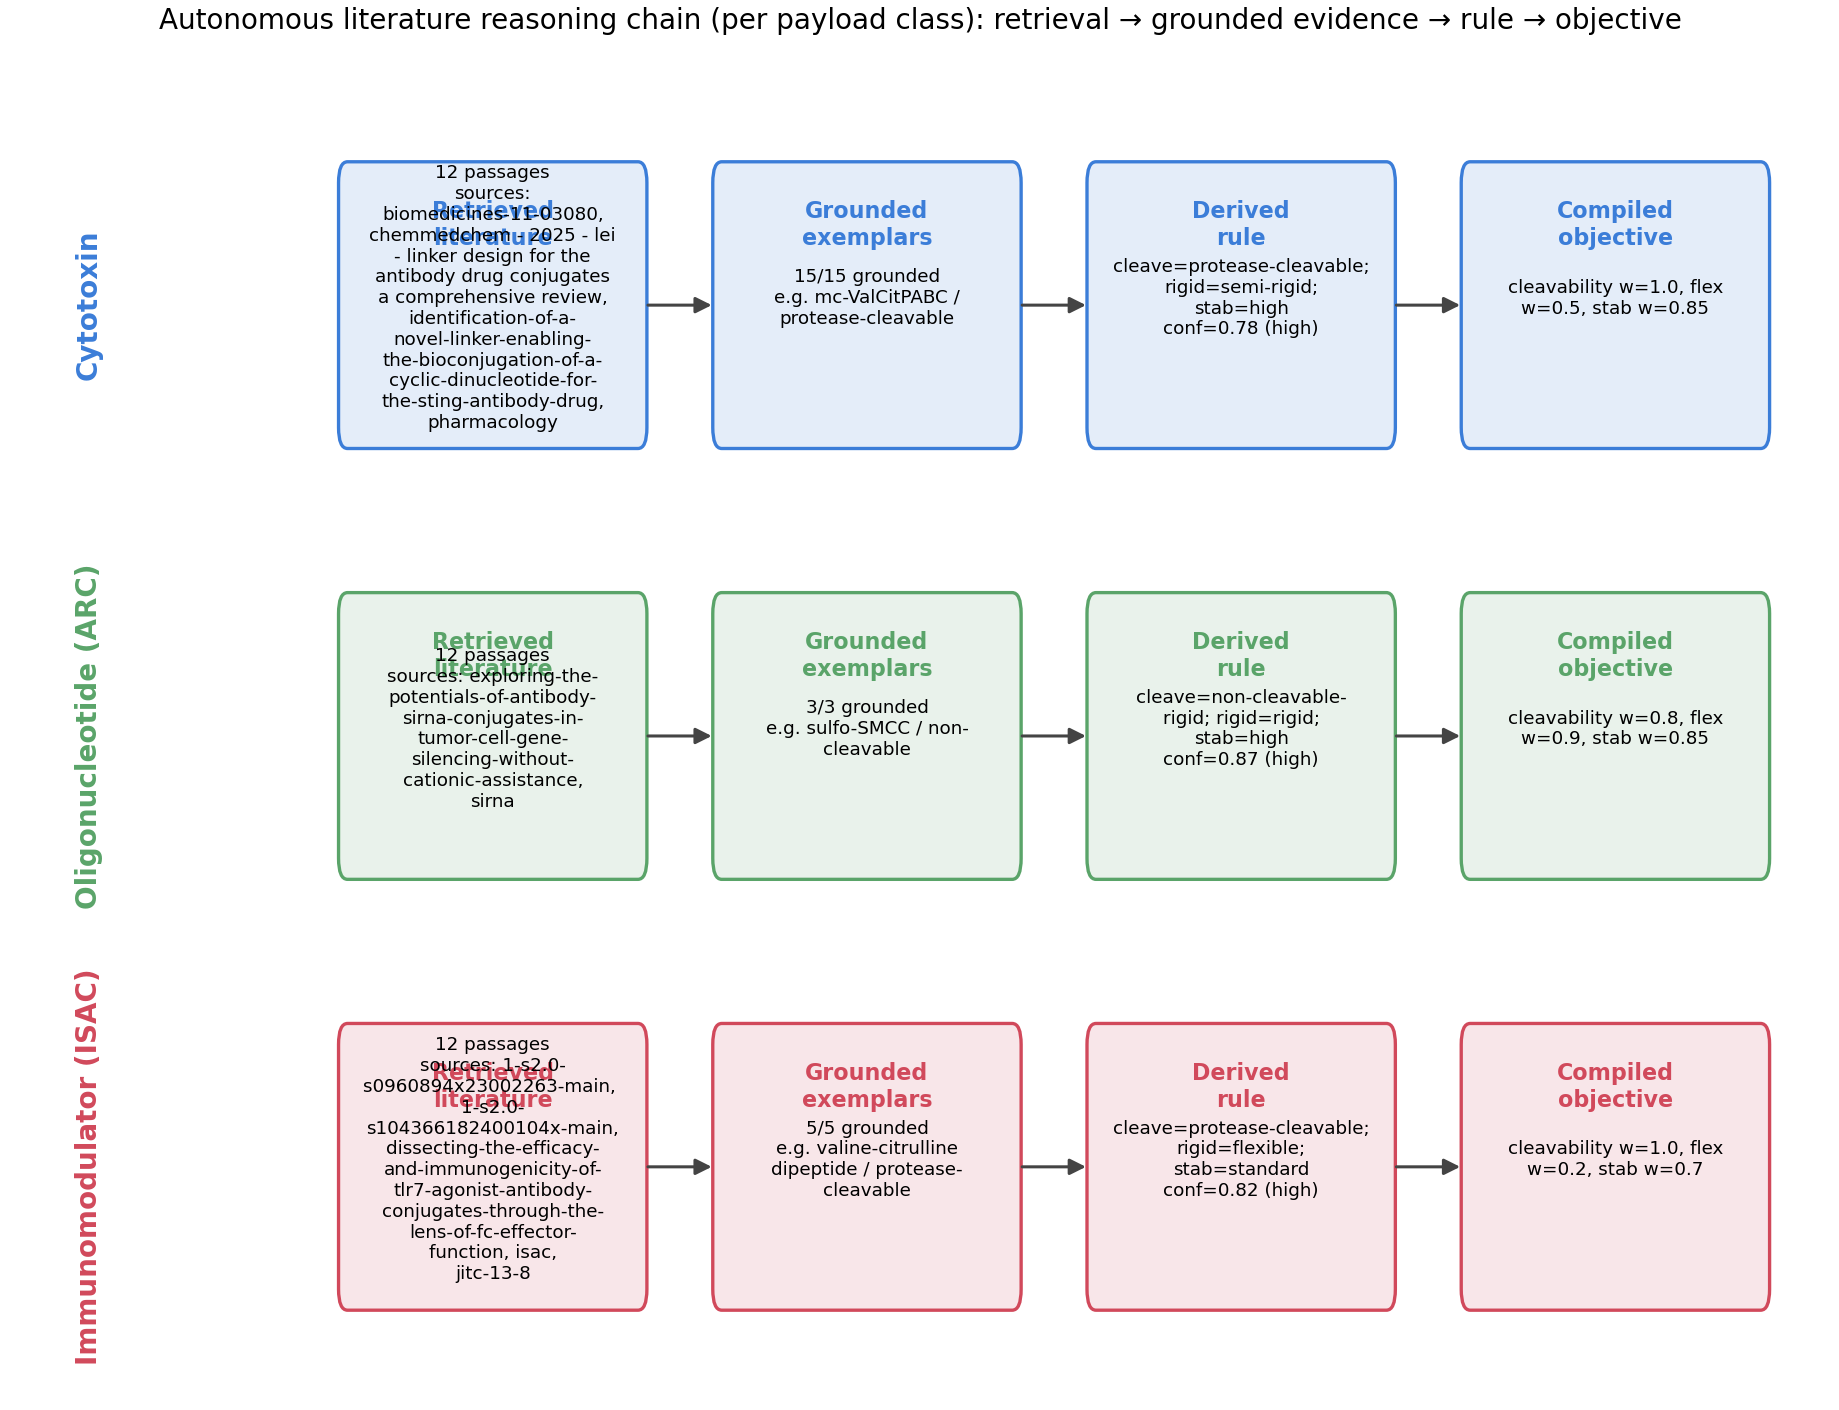
\includegraphics[width=0.80\linewidth]{fig_reasoning_cascade.png}\caption{The literature reasoning chain, per class: retrieval $\rightarrow$ grounded exemplars $\rightarrow$ derived rule (with confidence) $\rightarrow$ compiled objective, which then \emph{generates} the linkers. Every exemplar cites a retrieved passage.}\label{fig:chain}\end{figure}
\section{Methods}\subsection{Retrieval-grounded reasoning that drives generation}
For each payload class a literature agent (Claude Opus, LLM always on) queries a RAG store of 31 primary papers, retrieves passages with provenance, extracts exemplars that must each cite a retrieved passage (ungrounded ones are dropped), and derives a rule (cleavage/rigidity/stability) with a confidence---\emph{no} hardcoded fallback, so a failed call is an explicit abstain. The rule compiles deterministically into an ADC goal profile (cleavage regime, rotatable-bond window, per-term weights) that parameterises the REINVENT4 LinkInvent objective. \textbf{The compiled objective then generates the linkers} (staged learning, 40 steps, remote GPU box): the class-specific trigger warhead (Val-Cit-PABC, Val-Ala-PABC, or the rigid sulfo-SMCC cap) is welded into every molecule, so designs honour the derived motif, not just its regime.

\subsection{Honest scorers and a provenance gate}
Synthesizability is the continuous Ertl SA\_Score---the same metric the generator optimises---not a discretized step ladder; the step count survives only as a reported \emph{complexity index}. Plasma stability is mechanism-resolved (peptide/disulfide/maleimide/hydrolysis). Every value that reaches this paper is tagged \emph{measured} (a real model run: Boltz, REINVENT), \emph{llm}, or \emph{heuristic}; a gate refuses any \emph{mock}/default constant into a results claim, and the full provenance table is in the SI.

\subsection{Leave-one-paper-out}
We withhold a class's key paper(s), re-derive the rule from the remaining corpus, record the prediction and confidence \emph{before} revealing the withheld paper, and report agree/disagree. The withheld passages never enter retrieval.

\subsection{Structural co-fold}
We co-fold each designed linker with its real payload against cathepsin~B (Boltz-2) as two co-present ligands---an honest structural-plausibility check of \emph{recognition}, not a covalent whole-conjugate and not a claim of cleavage.
\section{Results}\subsection{The reasoning is visible, and it drives generation}
The agent grounded 23 exemplars in retrieved passages (Figure~\ref{fig:chain}) and compiled each rule into an objective that then \emph{generated} the molecules: 75 linkers were produced across the three classes, and the shortlisted designs carry the derived motif by construction---cytotoxins the Val-Cit dipeptide, ISACs the higher-stability Val-Ala, ARCs the rigid cyclohexane (sulfo-SMCC) cap (Table~\ref{tab:dossier}, Figure~\ref{fig:gallery}). This closes the loop the prior iteration left open: the delivered molecules are made by the agent's reasoning, not selected from a cached pool.

\subsection{Held-out test: robust rules versus a contested one}
Leave-one-paper-out does not merely confirm---it discriminates (Table~\ref{tab:heldout}, Figure~\ref{fig:heldout}). The cytotoxin and ISAC rules are \emph{robust}: withholding a paper leaves the agent deriving the same cleavable rule at high confidence (0.96, 0.83), because the literature agrees. The oligonucleotide rule is \emph{contested}. With the full corpus the top-retrieved siRNA-conjugate papers yield rigid non-cleavable (the sulfo-SMCC result). But withhold those, and from the \emph{remaining} ARC literature---modern clinical antibody-oligonucleotide conjugates such as DYNE-101/251 and AOC-1001---the agent confidently derives the \emph{opposite} rule: protease-cleavable Val-Cit (confidence 0.81, nine grounded exemplars). This is not a failure; it is the honest state of the science. Early cationic-assistance-free siRNA conjugates favour rigid non-cleavable linkers, while clinical AOCs increasingly use cleavable Val-Cit. A lookup-table agent would have hidden this; ours surfaces it, and its confidence tracks the evidence it is given---the strongest possible evidence that the conclusions are literature-derived, not encoded.

\begin{table}[t]\centering\caption{Leave-one-paper-out discriminates robust from contested rules. Direction is the derived cleavage preference; the ARC rule flips because the broader literature genuinely disagrees with the withheld siRNA paper.}\label{tab:heldout}\small
\begin{tabular}{l l c c c}\toprule
Class & Withheld & Full corpus & Held-out & Outcome \\ \midrule
Cytotoxin & biomedicines-11-03080 & cleavable (0.78) & cleavable (0.96) & robust \\
Immunomodulator (ISAC) & Immuno & cleavable (0.82) & cleavable (0.83) & robust \\
Oligonucleotide (ARC) & siRNA, exploring-the-poten & non-cleavable (0.87) & cleavable (0.81) & contested \\
\bottomrule\end{tabular}\end{table}

\subsection{Actionable, generated designs}
Figure~\ref{fig:gallery} draws the top generated designs with the conjugation handle (blue), scissile bond (red) and solubilising groups (green) detected programmatically. Table~\ref{tab:dossier} lists the fifteen designs; each is expanded into a dossier (route, cost, probability of success, failure modes, validation) in the SI. We report the heuristic complexity index honestly---peptidic Val-Cit linkers score high on it yet are clinically standard, a known limitation of count-based proxies.

\subsection{Structural co-fold}
All designs co-fold into the cathepsin~B cleft (ipTM 0.74--0.88); predicted $K_\mathrm{d}$ spans 9--109\,nM, with the Val-Cit cytotoxin design and the clinical mc-Val-Cit-PABC substrate (9 and 35\,nM) among the tighter binders---consistent with protease recognition, though affinity is not cleavage. We frame this as substrate recognition of two co-present ligands, not a covalent whole-conjugate.
\begin{figure}[t]\centering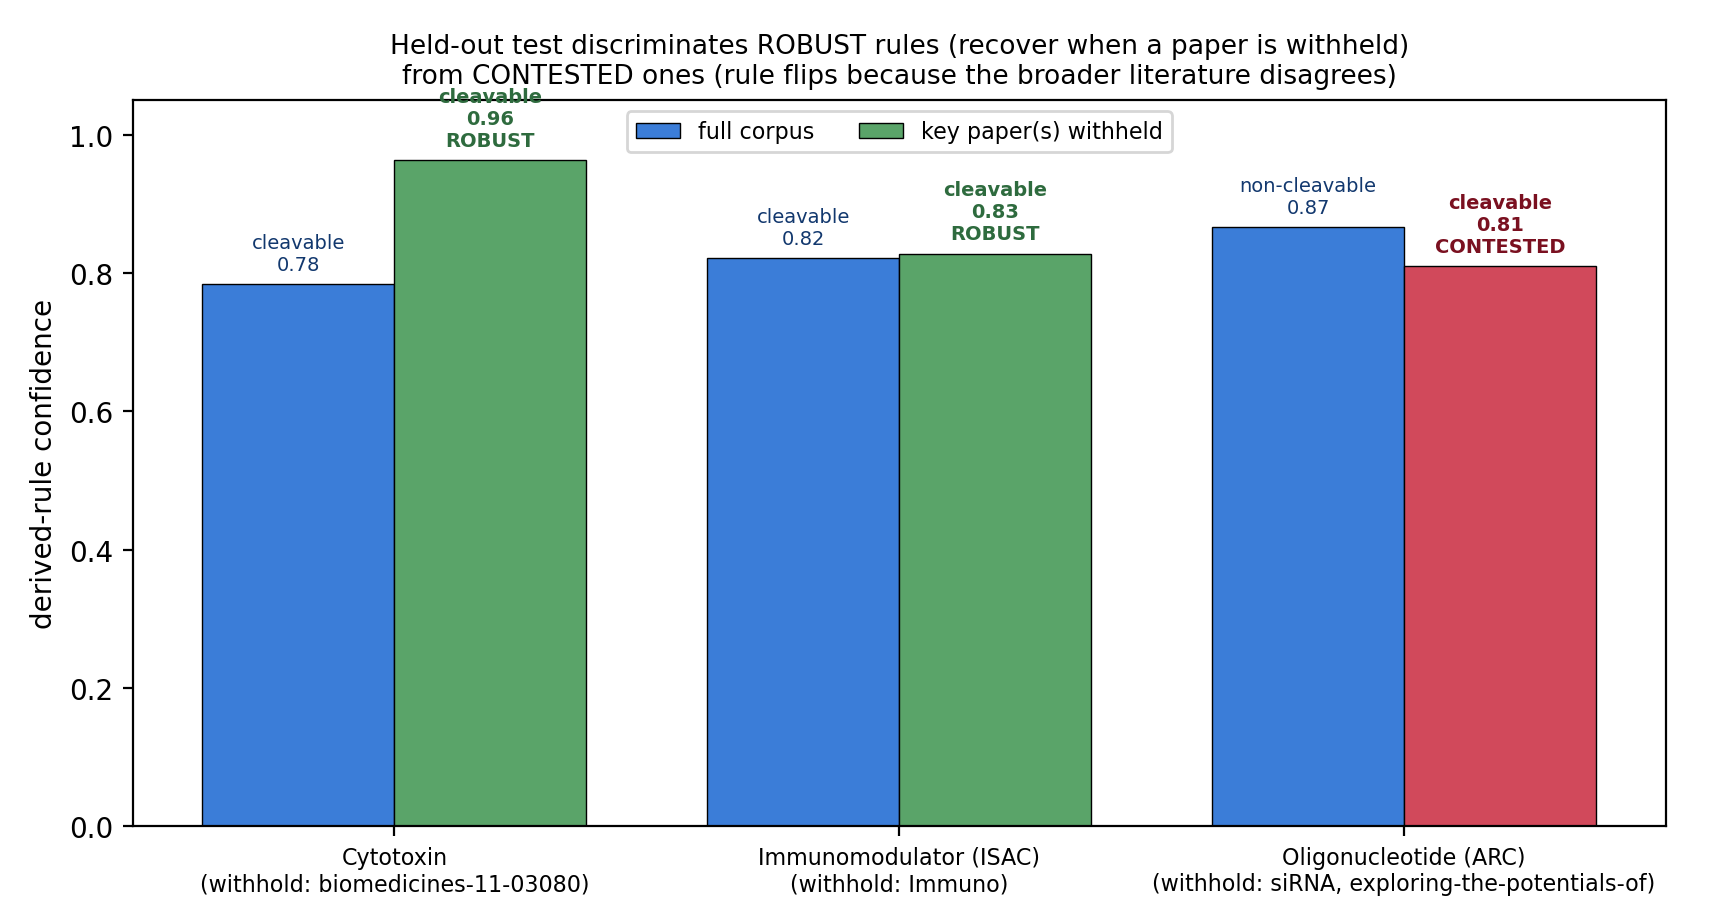
\includegraphics[width=0.72\linewidth]{fig_heldout.png}\caption{Leave-one-paper-out discriminates robust rules (cytotoxin, ISAC: recover at 0.96/0.83) from a contested one (ARC: flips non-cleavable$\rightarrow$cleavable at 0.81, because the clinical AOC literature disagrees with the withheld siRNA paper).}\label{fig:heldout}\end{figure}
\begin{figure}[t]\centering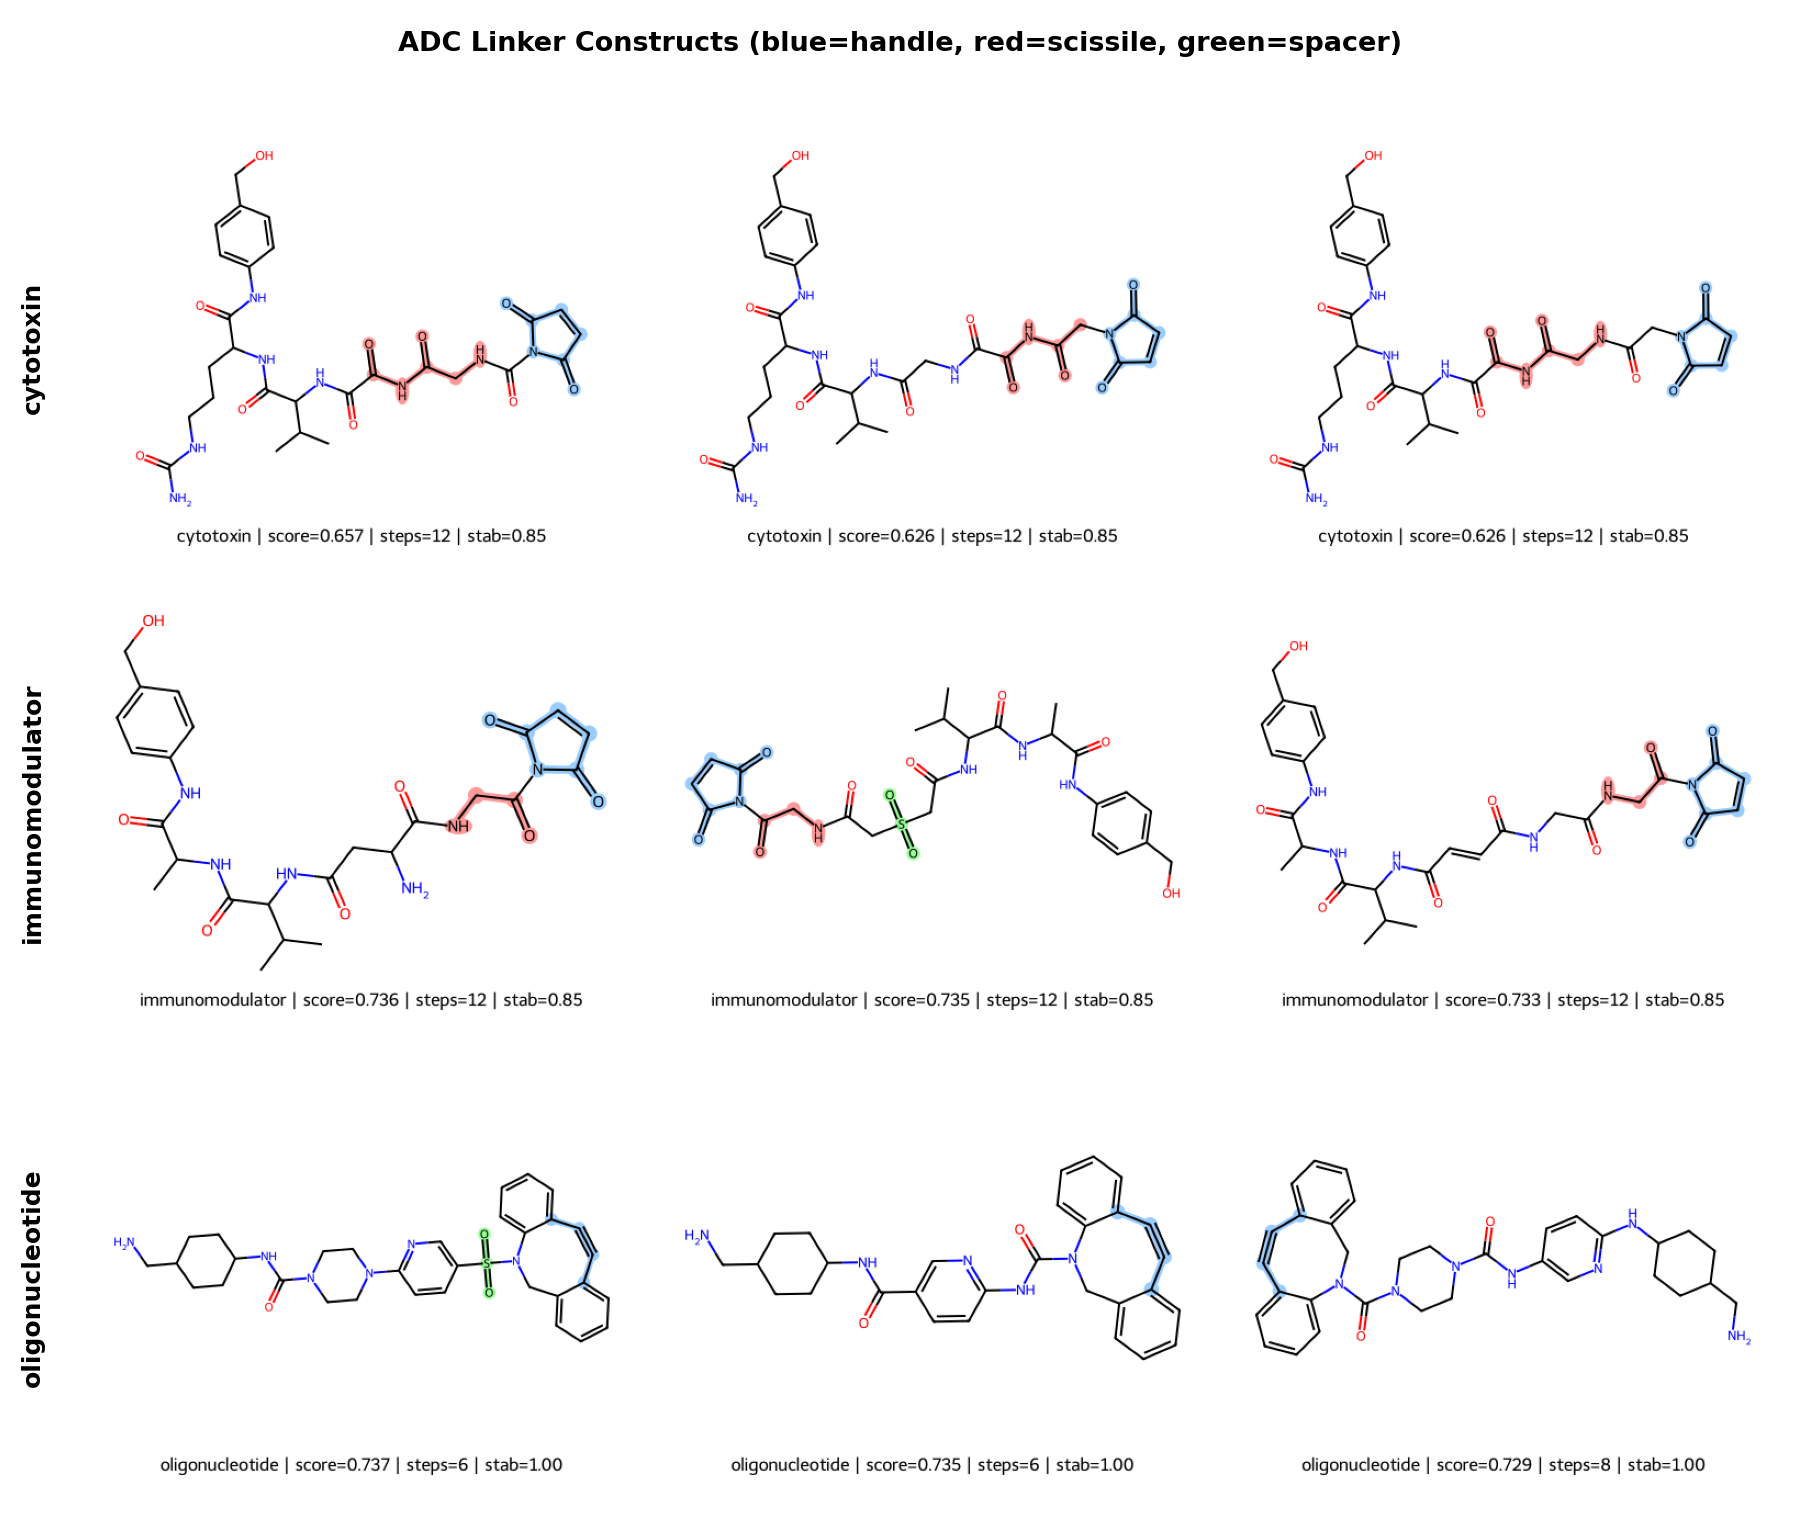
\includegraphics[width=0.80\linewidth]{structure_gallery.png}\caption{Top generated designs per class (handle blue, scissile bond red, solubiliser green; detected by SMARTS). Cytotoxin/ISAC carry the Val-Cit/Val-Ala motif; ARC carries the rigid cap.}\label{fig:gallery}\end{figure}
\begin{table}[t]\centering\caption{The fifteen \emph{generated} designs (5/class), produced by each class's compiled objective. Complexity index reported honestly (peptidic linkers score high yet are clinically standard). Full dossiers in the SI.}\label{tab:dossier}\scriptsize
\begin{tabular}{l l c c l c}\toprule
Class & Generated linker (SMILES) & Cplx.\ idx & Stab. & Nearest clinical (Tc) & P(succ) \\ \midrule
cytot & \texttt{CC(C)C(NC(=O)C(=O)NC(=O)CNC\ldots{}} & 12 & 0.85 & mc-Val-Cit-PABC (0.654) & 0.14 \\
cytot & \texttt{CC(C)C(NC(=O)CNC(=O)C(=O)NC\ldots{}} & 12 & 0.85 & mc-Val-Cit-PABC (0.711) & 0.14 \\
cytot & \texttt{CC(C)C(NC(=O)C(=O)NC(=O)CNC\ldots{}} & 12 & 0.85 & mc-Val-Cit-PABC (0.688) & 0.14 \\
cytot & \texttt{CC(C)C(NC(=O)C(=O)NC(=O)CN(\ldots{}} & 12 & 0.85 & mc-Val-Cit-PABC (0.654) & 0.14 \\
cytot & \texttt{CC(C)C(NC(=O)CC(=O)NC(=O)C(\ldots{}} & 12 & 0.85 & mc-Val-Cit-PABC (0.73) & 0.14 \\
immun & \texttt{CC(NC(=O)C(NC(=O)CC(N)C(=O)\ldots{}} & 12 & 0.85 & mc-Val-Ala-PABC (0.58) & 0.14 \\
immun & \texttt{CC(NC(=O)C(NC(=O)CS(=O)(=O)\ldots{}} & 12 & 0.85 & mc-Val-Ala-PABC (0.588) & 0.14 \\
immun & \texttt{CC(NC(=O)C(NC(=O)C=CC(=O)NC\ldots{}} & 12 & 0.85 & mc-Val-Ala-PABC (0.549) & 0.14 \\
immun & \texttt{CC(NC(=O)C(NC(=O)CCC(=O)NCC\ldots{}} & 12 & 0.85 & mc-Val-Ala-PABC (0.646) & 0.14 \\
immun & \texttt{CC(NC(=O)C(NC(=O)C(N)CCC(=O\ldots{}} & 12 & 0.85 & mc-Val-Ala-PABC (0.563) & 0.14 \\
oligo & \texttt{NCC1CCC(NC(=O)N2CCN(c3ccc(S\ldots{}} & 6 & 1.0 & MCC (non-cleava (0.145) & 0.65 \\
oligo & \texttt{NCC1CCC(NC(=O)c2ccc(NC(=O)N\ldots{}} & 6 & 1.0 & MCC (non-cleava (0.158) & 0.65 \\
oligo & \texttt{NCC1CCC(Nc2ccc(NC(=O)N3CCN(\ldots{}} & 8 & 1.0 & MCC (non-cleava (0.152) & 0.4 \\
oligo & \texttt{NCC1CCC(NC(=O)c2cnc(-c3cnc(\ldots{}} & 5 & 1.0 & MCC (non-cleava (0.16) & 0.85 \\
oligo & \texttt{NCC1CCC(NS(=O)(=O)N2CCN(C(=\ldots{}} & 5 & 1.0 & MCC (non-cleava (0.163) & 0.85 \\
\bottomrule\end{tabular}\end{table}
\section{Discussion}This iteration closes the gap between the thesis and the pipeline: the derived rule now \emph{makes} the molecules, and every number is provenance-tagged so no mock constant can reach a result. The headline is honest and, we think, more interesting than a clean recovery: the held-out test reveals that the ARC linker-cleavability rule is contested, with the agent confidently deriving cleavable Val-Cit from the clinical AOC literature once the early siRNA paper is withheld. \emph{Limitations.} The complexity index is a count-based proxy, not a route search (AiZynthFinder is the planned upgrade); the Boltz co-fold places linker and payload as co-present ligands, not a covalent construct; and the RAG is lexical. None of these are hidden---each is tagged and stated.
\section{Conclusion}An autonomous agent read 31 ADC papers, derived payload-class rules with grounded, confidence-annotated reasoning, used those rules to \emph{generate} synthesisable linkers, and, under a held-out test, distinguished robust rules from a genuinely contested one---surfacing an unresolved question in ARC linker design rather than papering over it. The framework generalises toward an autonomous medicinal-chemistry scientist that reasons, designs, and reports its own uncertainty. Provenance table, full chains, held-out details and all fifteen dossiers are in the SI.
\begin{thebibliography}{9}
\bibitem{su2021} Su, Z.; et al. Antibody--drug conjugates: Recent advances in linker chemistry. \emph{Acta Pharm. Sin. B} \textbf{2021}, 11 (12), 3889--3907.
\bibitem{balamkundu2023} Balamkundu, S.; Liu, C.-F. Lysosomal-Cleavable Peptide Linkers in Antibody--Drug Conjugates. \emph{Biomedicines} \textbf{2023}, 11 (11), 3080.
\bibitem{peng2021} Peng, B.; et al. Stimulus-cleavable chemistry in controlled drug delivery. \emph{Chem. Soc. Rev.} \textbf{2021}, 50, 4737--4762.
\bibitem{su2021zhang} Su, D.; Zhang, D. Linker Design Impacts ADC Pharmacokinetics and Efficacy. \emph{Front. Pharmacol.} \textbf{2021}, 12, 687926.
\bibitem{arc2025} Antibody--siRNA conjugates for tumor cell gene silencing without cationic assistance. \emph{Bioconjugate Chem.} \textbf{2025}. DOI: 10.1021/acs.bioconjchem.5c00212.
\bibitem{isac2022} Immune-stimulating antibody conjugates elicit robust myeloid activation (TLR7/8 ISAC). \emph{Mol. Pharmaceutics} \textbf{2022}. DOI: 10.1021/acs.molpharmaceut.2c00392.
\bibitem{isac2025} Design of TLR7/8 agonist immune-stimulating antibody conjugates with tuned linker cleavability. \emph{J. Med. Chem.} \textbf{2025}. DOI: 10.1021/acs.jmedchem.5c01908.
\bibitem{boltz2} Passaro, S.; et al. Boltz-2: Towards accurate and efficient binding-affinity prediction. \textbf{2025}.
\end{thebibliography}

\end{document}